\subsection{Background}
There is no previous progress to refer to, as the machine learning roles of the Aerodynamic Test Platform and Wings (ATPW) subgroup are newly defined responsibilities.

\subsection{Introduction}
The overall goal for the neural network is to develop a non-linear black-box aerodynamic model using a machine learning model to predict three-dimensional aerodynamic forces to validate and compare with the 
experimental data obtained from the Aerodynamic Test Platform (ATP). Eventually, for comparison, two different machine learning approaches, such as neural networks, will be used to model the non-linear aerodynamics of flapping wings. The team has currently collected aerodynamic data on NACA airfoils to synthesize and validate aerodynamic models as a preliminary exercise.

\subsection{Analysis of Problem}
Before steps could be taken towards developing a model, an understanding of machine learning (ML) to a certain level had to be established. This was done through online resources, for example, online lectures presented by Andrew Ng at Stanford \cite{NgDeepLearningPlaylist2025}, YouTube video series such as Deep Learning With Tensorflow 2.0, Keras and Python by codebasics \cite{codebasicsDeepLearning2025}, podcasts such as the Machine Learning Guide by OCDevel \cite{OCDevelMLGSpotify2025}, discussions with the assigned Lead Engineer Professor Hashim A. Hashim Mohamed, and more. For future groups, Andrew Ng's Coursera course was also often recommended.

\subsubsection{Dataset Preparation}
Before a machine model could be selected and created, a dataset needed to be selected. NACA airfoil data were chosen for the preliminary exercise. The NACA airfoil data were selected because there appeared to be some rough correlation and potential overlap between the categories of data presented for the NACA airfoils and the potential data to be extracted from the Micro Flapping-Wing Flyer (MFWF) and ATP. Joukowsky and NACA 4, 5, 6, and 7 digit airfoil data were extracted from airfoiltools.com \cite{AirfoilToolsNACA4Digit2025}. Each airfoil on airfoiltools.com was divided into seven files, each containing data for one of the seven Reynolds-number intervals from 50,000 to 5,000,000. Initially, to develop the ML model, a small sample of airfoil data was downloaded as a Microsoft Excel file and combined to enable faster training and iteration. Over time, as the ML model was developed, Aidan Sheridan compiled a large Excel dataset containing all available airfoils and associated information, adding two new columns: one for the NACA Airfoil ID and another for the Reynolds Number. A few refinements were applied to the large dataset to make it easier for the ML model to read, and the model was then trained on it. There are six categories of information that were available with each NACA airfoil: angle of attack (\( \alpha \)), transition point on upper and lower surface (Top\_Xtr and Bot\_Xtr), Reynolds Number (Re), lift coefficient (Cl), drag coefficient (Cd), pitching moment (Cm), and profile drag coefficient (Cdp).

\subsubsection{Machine Learning Model Development}
The machine learning (ML) model for the preliminary exercise was to predict / output four values, the lift coefficient (Cl), drag coefficient (Cd), pitching moment (Cm), and profile drag coefficient (Cdp) based on five input parameters, NACA airfoil ID, angle of attack (\( \alpha \)), transition point on upper and lower surface (Top\_Xtr and Bot\_Xtr), and Reynolds Number (Re).

The initial ML approach led to the development of a Long Short-Term Memory (LSTM), a type of Recurrent Neural Network (RNN), as recommended based on in-class feedback. An LSTM model is designed for time-series/sequential data, data that depends on previous data points, streams of data. For example, predicting the weather depends on current and previous conditions and how they have changed over time. However, the NACA airfoil data is not sequential; it does not depend on the data before or after it. Each row of data is independent and can be randomly ordered; this would not affect the prediction. The LSTM model added complexity without improving prediction accuracy. Early tests showed that the LSTM model underperformed, particularly when the NACA airfoil ID was not used as an input parameter (four inputs instead of five) compared to other models discussed later. LSTMs require 3-dimensional input (batch, time, and features). Since the NACA airfoil data was not sequenced, no time dimension, requiring the addition of a forced fake sequence that provided no meaningful context to the model, adding unnecessary complexity and slowing it down. Overall, the LSTM model had an increased training time, memory usage, and hyperparameter sensitivity.

A Multi-Layer Perceptron (MLP) model was trained as it was better suited to the NACA airfoil dataset. An MLP was chosen because the NACA airfoil data is not sequential; it is static. MLP models can take an input of a simple list of numbers and learn relationships among them. The aerodynamic coefficients being predicted depend on complex interactions among variables, and MLP models can learn these nonlinear patterns to a relatively high degree of accuracy. MLP models contain fewer layers and complications, resulting in a simpler architecture compared to the previous LSTM model.

\subsubsection{Model Evaluation and Validation}

To assess the accuracy of the trained model, two main plots are utilized. Figures~\ref{fig: LSTM 2: Pred vs True Coefficients} and~\ref{fig: MLP: Pred vs True Coefficients} depict the true coefficient as the x-coordinate and the associated models prediction as the y-coordinate. The line y=x represents where the predictions perfectly represent the true coefficient, and the farther the distance from the line, the worse the prediction is. Figures~\ref{fig: LSTM 2: Training Accuracy} and~\ref{fig:MLP: Training Accuracy} show the system's accuracy using mean squared error (MSE) loss as a function of Epoch, the number of times the model has gone through the dataset.

\begin{figure}[htbp]
    \centering
    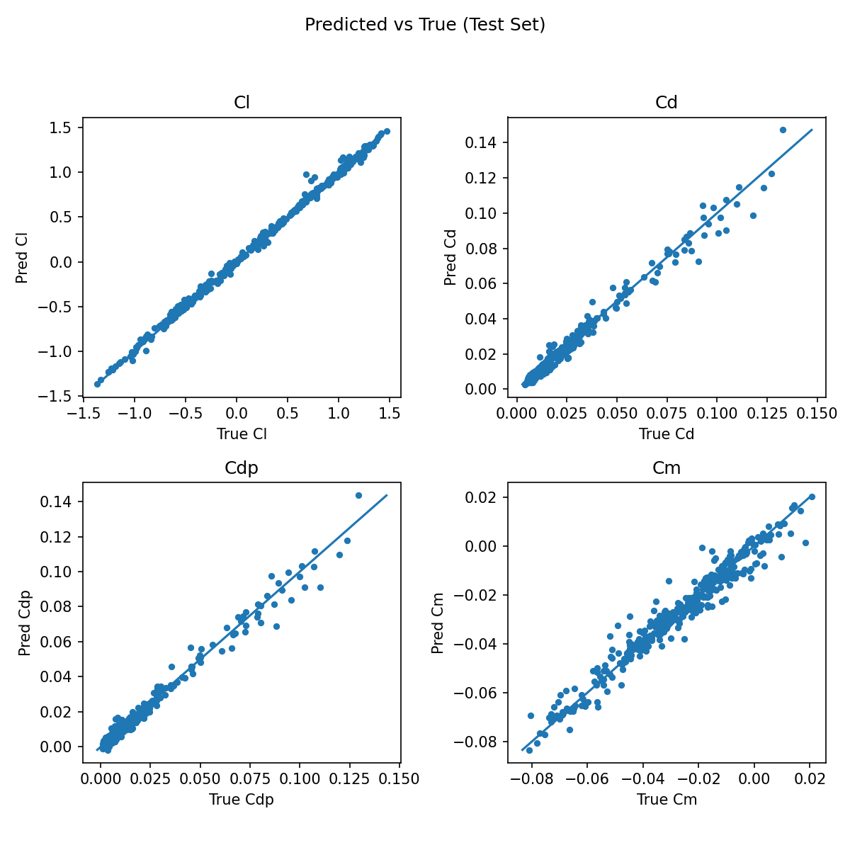
\includegraphics[width = 10 cm]{figures/Wade Schnurr Images/LSTM 2 Predicted vs True (Test Set).png}
    \caption{LSTM model version 2, predicted coefficient results compared to the actual coefficient values.}
    \label{fig: LSTM 2: Pred vs True Coefficients}
\end{figure}

\begin{figure}[htbp]
    \centering
    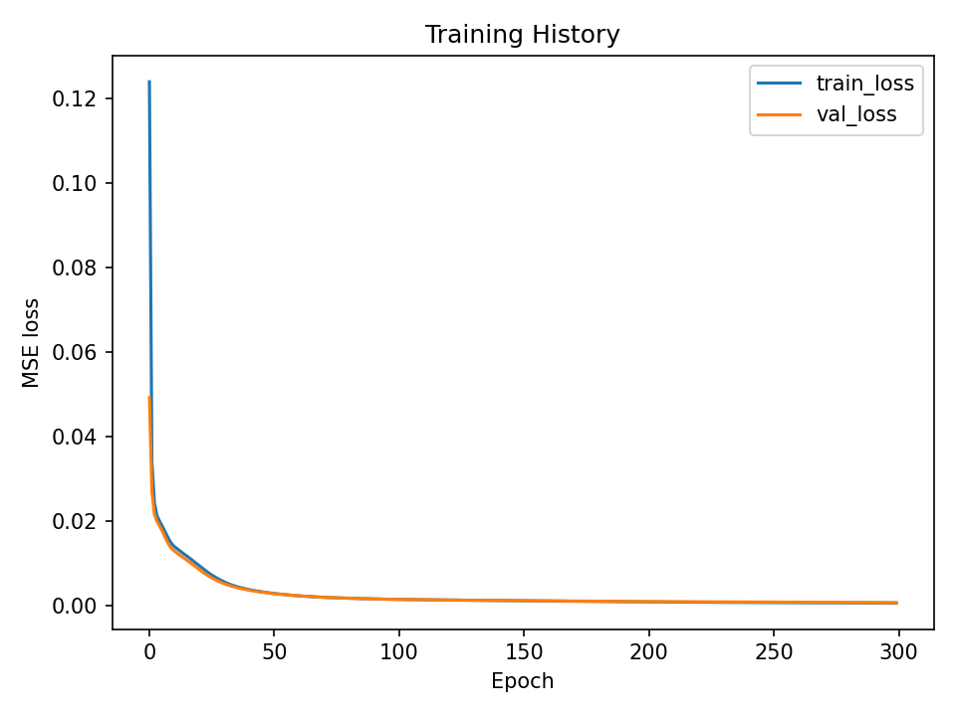
\includegraphics[width = 10 cm]{figures/Wade Schnurr Images/LSTM 2 with Arifoil Training History.png}
    \caption{LSTM model version 2, training accuracy compared to the number of times the dataset has been run through.}
    \label{fig: LSTM 2: Training Accuracy}
\end{figure}

\begin{figure}[htbp]
    \centering
    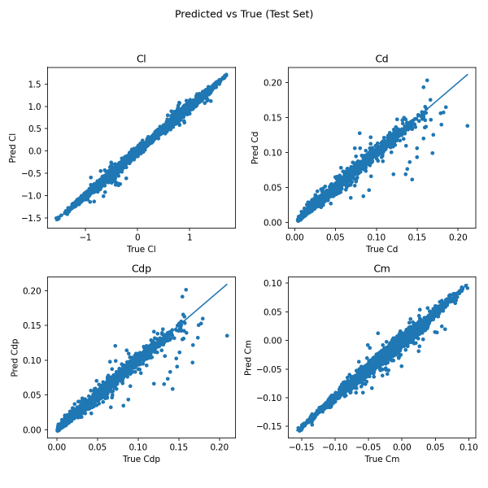
\includegraphics[width = 10 cm]{figures/Wade Schnurr Images/MLP Predicted vs True (Test Set).png}
    \caption{MLP model predicted coefficient results compared to the actual coefficient values.}
    \label{fig: MLP: Pred vs True Coefficients}
\end{figure}

\begin{figure}[htbp]
    \centering
    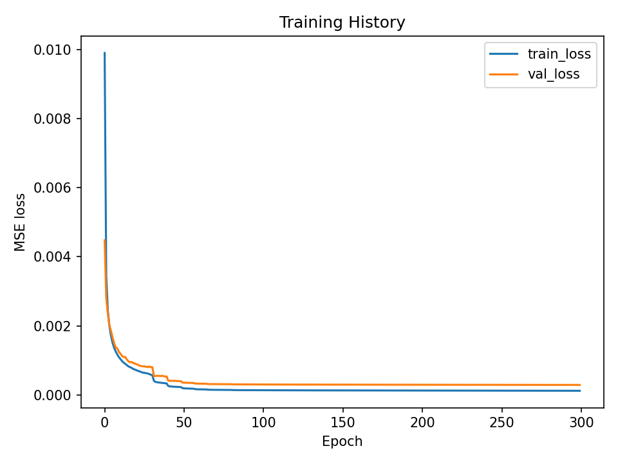
\includegraphics[width = 10 cm]{figures/Wade Schnurr Images/MLP Training History (Large NACA Airfoil Dataset).png}
    \caption{MLP model training accuracy compared to the number of times the large dataset has been run through.}
    \label{fig:MLP: Training Accuracy}
\end{figure}

\newpage
\subsection{Plan for Winter Semester}
At this time, there are two main goals for the ATPW machine learning group to continue progress into the winter semester. One: determine relevant ways to interpret and display the information generated by the current MLP model trained on NACA airfoil data. Two: consider the data that will be used as inputs and outputs from the ATP, how the X, Y, and Z forces are produced and their format. Analyze whether the current MLP model can be modified to accept the information from the ATP and produce high-accuracy results, or if it is necessary to develop a new model better suited for the type of data generated by the ATP.